
\documentclass[12pt]{article}

\usepackage{amsmath}
\allowdisplaybreaks
\usepackage{amsthm}
\usepackage{amssymb}
\usepackage[colorlinks=true]{hyperref}
\usepackage{tikz}
% \usepackage{apalike}
\usepackage{natbib}

\usetikzlibrary{bayesnet}

\newtheorem{lemma}{Lemma}
\newtheorem{theorem}{Theorem}

\title{Derivation of the Kalman filter equations}
\author{Joaquín Rapela}

\begin{document}

\maketitle

\begin{theorem}

    Given the linear dynamical systems model

    \begin{alignat*}{2}
        \mathbf{x}_{t+1}&=A_t\mathbf{x}_t+\mathbf{w}_t&\quad&\text{with }\mathbf{w}_t\sim N(0,Q_t)\\
        \mathbf{y}_t&=B_t\mathbf{x}_t+\mathbf{v}_t&&\text{with }\mathbf{v}_t\sim N(0,R_t)\\
        \mathbf{x}_0&\sim N(\mathbf{m}_0,V_0)&&
    \end{alignat*}

    \noindent (represented in Fig.~\ref{fig:ldsModel}), then the predictive
    distribution, $p(\mathbf{x}_t|\mathbf{y}_1,\ldots,\mathbf{y}_{t-1})$, and
    the filtering distribution,
    $p(\mathbf{x}_t|\mathbf{y}_1,\ldots,\mathbf{y}_t)$, are

    \begin{align*}
        p(\mathbf{x}_t|\mathbf{y}_1,\ldots,\mathbf{y}_{t-1})&=N(\mathbf{x}_t|\mathbf{x}_{t|t-1},P_{t|t-1})\\
        p(\mathbf{x}_t|\mathbf{y}_1,\ldots,\mathbf{y}_t)&=N(\mathbf{x}_t|\mathbf{x}_{t|t},P_{t|t})
    \end{align*}

    \noindent with

    \begin{align*}
        \mathbf{x}_{t|t-1}&=A_{t-1}\mathbf{x}_{t-1|t-1}\\
        P_{t|t-1}&=A_{t-1}P_{t-1|t-1}A_{t-1}^\intercal+Q_{t-1}\\
        \hat{\mathbf{y}}_{t|t-1}&=B_t\mathbf{x}_{t|t-1}\\
        \mathbf{z}_t&=\mathbf{y}_t-\hat{\mathbf{y}}_{t|t-1}\\
        S_t&=\text{Cov}(\{\mathbf{z}_t\}|\mathbf{y}_1,\ldots,\mathbf{y}_{t-1})=B_tP_{t|t-1}B_t^\intercal+R_t\\
        \mathbf{x}_{t|t}&=\mathbf{x}_{t|t-1}+K_t\mathbf{z}_t\\
        \mathbf{P}_{t|t}&=(I-K_tB_t)P_{t|t-1}\\
        \mathbf{K}_t&=P_{t|t-1}B_t^\intercal S_t^{-1}\\
        \mathbf{x}_{0|0}&=\mathbf{m}_0\\
        P_{0|0}&=V_0
    \end{align*}
    \label{thm:kalmanFilterEqs}
\end{theorem}

The following proof adds a few more details to that given in Section 4.3.1 of
\citet{durbinAndKoopman12}.

\begin{proof}
    Call $Y_t=\{\mathbf{y}_1,\ldots,\mathbf{y}_t\}$, then

    \begin{align}
        \mathbf{x}_{t|t-1}&=E\{\mathbf{x}_t|Y_{t-1}\}=E\{A_{t-1}\mathbf{x}_{t-1}+\mathbf{w}_{t-1}|Y_{t-1}\}\nonumber\\
                          &=A_{t-1}E\{\mathbf{x}_{t-1}|Y_{t-1}\}+E\{\mathbf{w}_{t-1}|Y_{t-1}\}\nonumber\\
                          &=A_{t-1}\mathbf{x}_{t-1|t-1}+E\{\mathbf{w}_{t-1}\}=A_{t-1}\mathbf{x}_{t-1|t-1}\label{eq:p1n1}
    \end{align}

\end{proof}

Notes:
\begin{enumerate}
    \item the first equality in Eq.~\ref{eq:p1n1} holds because
        $\mathbf{w}_{t-1}$ is independent of $Y_{t-1}$.
\end{enumerate}

\begin{figure}
    \centering
    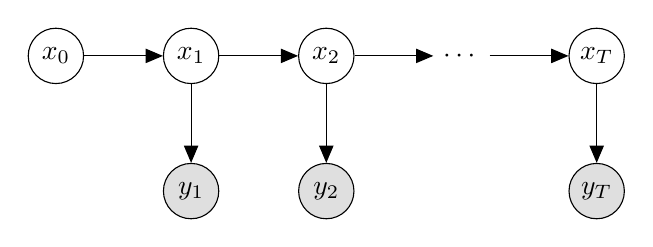
\begin{tikzpicture}[node distance=2.5cm and 1.8cm]

  % Nodes for hidden states
  \node[latent]              (x0) {$x_0$};
  \node[latent, right=of x0] (x1) {$x_1$};
  \node[latent, right=of x1] (x2) {$x_2$};
  \node[latent, right=of x2, draw=none] (xD) {$\cdots$};
  \node[latent, right=of xD] (xT) {$x_T$};

  % Nodes for observations
  \node[obs, below=of x1] (y1) {$y_1$};
  \node[obs, below=of x2] (y2) {$y_2$};
  \node[obs, below=of xT] (yT) {$y_T$};

  % Edges between hidden states
  \edge {x0} {x1};
  \edge {x1} {x2};
  \edge {x2} {xD};
  \edge {xD} {xT};

  % Emission edges
  \edge {x1} {y1};
  \edge {x2} {y2};
  \edge {xT} {yT};

\end{tikzpicture}

    \caption{Graphical models for our linear dynamical system in
    Theorem~\ref{thm:kalmanFilterEqs}.}
    \label{fig:ldsModel}
\end{figure}

\documentclass[12pt]{article}

\usepackage{amsmath}
\usepackage{theorem}

\newtheorem{theorem}{Theorem}

\title{Conditional distribution for jointly normal Gaussian random variables}
\author{Joaquín Rapela}

\begin{document}

\maketitle

\begin{theorem}

    Let $\mathbf{x}$ and $\mathbf{y}$ be jointly normally-distributed random
    vectors with

    \begin{align*}
        E\left\{\left(\begin{array}{c}
                          \mathbf{x}\\
                          \mathbf{y}
                      \end{array}\right)\right\}&=\left(\begin{array}{c}
                                                           \boldsymbol{\mu}_x\\
                                                           \boldsymbol{\mu}_y
                                                       \end{array}\right)\\
        \text{Cov}\left\{\left(\begin{array}{c}
                                   \mathbf{x}\\
                                   \mathbf{y}
                               \end{array}\right)\right\}&=\left(\begin{array}{cc}
                                                                     \Sigma_{xx} & \Sigma_{xy} \\
                                                                     \Sigma_{yx} & \Sigma_{yy} \\
                                                                  \end{array}\right)
    \end{align*}

    \noindent where $\Sigma_{yy}$ is assumed to be non-singular.
    %
    Then the conditional distribution of $\mathbf{x}$ given $\mathbf{y}$ is
    normal with mean vector

    \begin{align*}
        \text{E}\{\mathbf{x}|\mathbf{y}\}=\boldsymbol{\mu}_x+\Sigma_{xy}\Sigma_{yy}^{-1}(\mathbf{y}-\boldsymbol{\mu}_y)
    \end{align*}

    \noindent and covariance matrix

    \begin{align*}
        \text{Cov}\{\mathbf{x}|\mathbf{y}\}=\Sigma_{xx}-\Sigma_{xy}\Sigma_{yy}^{-1}\Sigma_{yx}
    \end{align*}
\end{theorem}

\end{document}


\bibliographystyle{apalike}
\bibliography{linearDynamicalSystems}

\end{document}
